\documentclass[14pt]{article}
\usepackage{amsmath,amsthm,amssymb}

\usepackage[a4paper, top=2cm, bottom=2cm, left=3cm, right=1cm]{geometry}

\usepackage[T1,T2A]{fontenc}
\usepackage[utf8]{inputenc}
\usepackage[english,russian]{babel}

\usepackage{epsfig}

\usepackage{verbatim}

\usepackage{hyperref}
\hypersetup{
    colorlinks,
    citecolor=black,
    filecolor=black,
    linkcolor=black,
    urlcolor=black
}

\setcounter{secnumdepth}{4}
\setcounter{tocdepth}{6}

\begin{document}

\pagebreak

\clearpage
\setcounter{page}{3}

\tableofcontents

\pagebreak

\subsection*{Введение}
\addcontentsline{toc}{subsection}{Введение}

IEC 61499\footnote{\url{https://webstore.iec.ch/searchform&q=61499}} --
международный стандарт проектирования и разработки промышленных управляющих и
измерительных систем \cite{iec}. Спецификация этого стандарта определяет общую модель
распределенных систем управления и основана на стандарте
IEC 61131\footnote{\url{https://webstore.iec.ch/searchform&q=61131}}. Согласно
стандарту IEC 61499 программа представляется в виде сети функциональных блоков.
Для каждого функционального блока определен интерфейс, который задает набор
входных и выходных событий и переменных. Функциональные блоки могут быть
базисными и составными. Базисный функциональный блок описывется с помощью
диаграммы управления выполнением (\textit{execution control chart, ECC}), которая является специальной формой конечного
автомата Мура. Каждое состояние имеет несколько выходных действий. Каждое
действие может включать в исполнение выработку выходного события. Алгоритмы
изменяют значения выходных переменных. Составные блоки являются сетями соединенных
между собой блоков, как базисных так и составных.

В данной работе рассматривается восстановление логики базисного
функционального блока. Вместе с тем предложенные алгоритмы могут быть с небольшими изменениями
применены и к составным блокам.

Задача восстановления логики функционального блока возникает, когда исходный код
блока потерян и доступен только бинарный исполняемый файл. Представленный
в \cite{rec} подход позволяет восстановливать диаграммы управления выполнением при помощи
тестирования: исходный функциональный блок подвергается тестированию, его
поведение записывается в виде сценариев работы, и затем при помощи
методов оптимизации (например, эволюционных алгоритмов \cite{ea}) находится диаграмма, удовлетворяющая сценариям.

В этом подходе, однако, возникает серьезный вопрос о полноте набора сценариев.
Не имея исходного кода, мы не можем гарантировать, что тесты покрывают все
необходимое поведение блока, а значит нет гарантий, что полученный блок будет
эквивалентен исходному даже с точки зрения поведения.

В данной работе предлагается подход к решению указанной проблемы с использованием верификации
функциональных блоков. Входные данные дополняются темпоральными свойствами,
которым удовлетворял исходный автомат. Эти свойства выражаются при помощи
темпоральных логик (например, линейной темпоральной логики (\textit{linear temporal logic, LTL})) и часто могут быть
выведены из документации или других источников. Предполагается, что эти
свойства описывают наиболее важные свойства блока. Таким образом, если 
гарантировать, что полученный блок удовлетворяет этим свойствам, то
основная функциональность будет сохранена.

Таким образом, целью данной работы является разработка метода генерации
функциональных блоков, для которых будет выполняться поведение, заданное
набором сценариев, а так же удовлетворяющих заданным темпоральным свойствам.

Представленный в данной работе подход основан на методе представленном в \cite{rec},
однако встраивает в процесс верификацию. Основными результатами данной работы
являются:

1) Подход для быстрой верификации функциональных блоков, лежащий между
верификацией замкнутого и открытого цикла.

2) Подход, комбинирующий тестирование и верификацию для синтеза функциональных
блоков.

В данной работе будем рассматривать только базисные функциональные блоки, в которых
все входные и выходные переменные являются булевыми.

\pagebreak

\subsection{Определения и постановка задачи}

\subsubsection{Метаэвристические алгоритмы}

Метаэвристические алгоритмы \cite{meh} являются классом оптимизационных методов,
позволяющих находить решения для широкого круга сложных задач. Они используются,
когда другие методы неприемлимы ввиду вычислительной затратности, и в частности
используются для решения некоторых NP-трудных задач. К метаэвристическим алгоритмам относятся, например,
эволюционные, генетические и муравьиные алгоритмы.

Эволюционные алгоритмы используют и моделируют процессы естественного отбора
для решения задачи. Все они моделируют базовые положения теории биологической
эволюции -- процессы отбора, мутации и воспроизводства. Поведение агентов
определяется окружающей средой. Множество агентов принято называть популяцией.
Такая популяция эволюционирует в соответствии с правилами отбора и целевой функцией, задаваемой окружающей средой.

Генетические алгоритмы схожи с эволюционными алгоритмами, но имеют акцент на
использовании оператора скрещивания.

В основе муравьиных алгоритмов лежит моделирование поведения муравьиной колонии.
В процессе поиска источников пищи муравьи откладывают на своем пути особое
химическое вещество -- феромон. Большая концентрация феромона на определенном участке пути
муравья привлекает его, увеличивая вероятность того, что муравей проложит свой путь через
эту область. Со временем феромон испаряется, и его концентрация уменьшается. Чем короче
путь муравья до источника пищи и обратно, тем меньше времени потребуется для его преодоления,
тем больше концентрация феромона на его пути, тем больше муравьев последуют этому пути.
Такой метод позволяет муравьям находить пути близкие к оптимальным с точки зрения длины.

\subsubsection{Конечно-автоматные модели}

Абстрактный конечный автомат является математической моделью дискретного устройства
и описывается шестеркой $\langle A, Z, W, \sigma, \lambda, a_0 \rangle$,
где $A$ -- конечное множество состояний, $Z$ -- множество входных сигналов,
$W$ -- множество выходных сигналов, $\sigma : A \times Z \rightarrow A$ --
функция переходов. $\lambda : A \times Z \rightarrow W$ -- функция выходов,
$a_0$  -- начальное состояние.

Существуют два вида абстрактных автоматов -- автоматы Мили и автоматы Мура.
В автоматах Мили выходные сигналы зависят от состояния и входного сигнала,
а в автоматах Мура только от состояния. В автоматах Мили
выходные сигналы записаны на переходах, а в автоматах Мура в состояниях.
На рисунках Рис. \ref{mili-example} и Рис. \ref{moor-example} изображены примеры
автоматов Мили и Мура. Состояния помечены как $a_i$, входные сигналы --
$z_i$, выходные сигналы -- $w_i$.

\begin{figure}
\centering
\begin{minipage}{.5\textwidth}
    \centering
    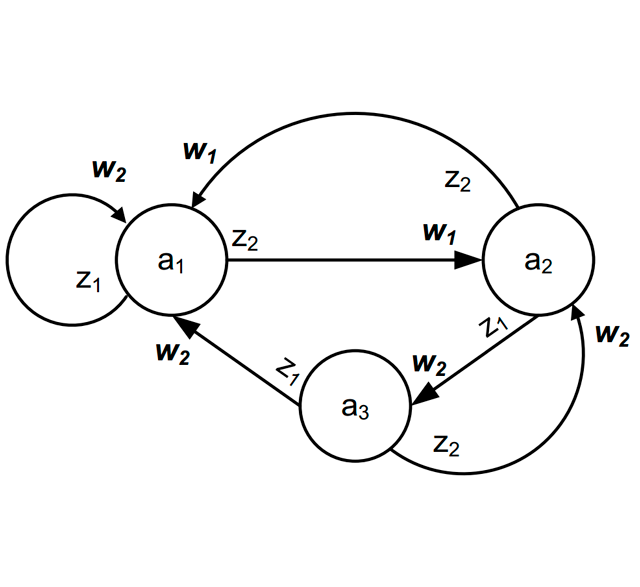
\includegraphics[width=2.5in]{pic/Aa_mili_ex2.png}
    \caption{Пример автомата Мили}
    \label{mili-example}
\end{minipage}%
\begin{minipage}{.5\textwidth}
    \centering
    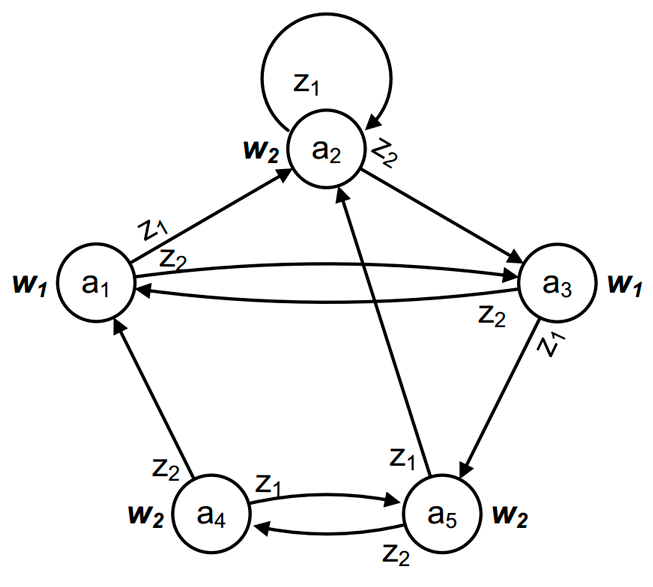
\includegraphics[width=2.5in]{pic/Aa_moor_ex1.png}
    \caption{Пример автомата Мура}
    \label{moor-example}
\end{minipage}
\end{figure}

\subsubsection{Стандарт IEC 61499}

В рамках стандарта IEC 61499 определяется архитектура распределенных систем управления.
Приложение определяется как сеть соединенных между собой функциональных блоков.
Используется событийная модель исполнения: блоки работают независимо и способны
обрабатывать и генерировать события, которые в свою очередь могут быть обработаны
другими блоками. Интерфейс функционального блока определяет входные и выходные события и переменные блока.
Пример интерфейса представлен на рисунке \ref{fb-interface-example}.
Базисный функциональный блок определяется в терминах диаграммы управления выполнением, которая является
автоматом Мура специального вида.
Составной функциональный блок определяется как сеть соединенных между собой функциональных блоков.

\subsubsection{Базисный функциональный блок}

Рассмотрим подробнее базисный функциональный блок так как именно он будет в
дальнейшем представлять для нас интерес.
Диаграммой управления выполнением в данной работе будем называть девятку $\langle E, I, Y, Z, O, y_0, \phi,
\sigma, \tau \rangle$, где $E$ -- множество входных событий, $I$ -- множество
входных булевых переменных, $Y$ -- множество состояний, $Z$ -- множество
выходных событий, $O$ -- множество выходных булевых переменных, $y_0$ --
начальное состояние, $\phi : Y \times E \times \{0, 1\}^{|I|} \rightarrow
Y$ -- функция переходов, $\sigma : Y \rightarrow Z^*$ -- функция выходных
событий и $\tau : Y \rightarrow \{0, 1, x\}^{|O|}$ -- функция значений
выходных переменных, где 0 и 1 означает присвоение соответствующего значения
переменной и $x$ означает сохранение ее текущего состояния. Пример диаграммы
управления выполнением представлен на рисунке \ref{ecc-example}.
В состояниях находятся алгоритмы, задающие значения выходных переменных, и
множества выходных событий, которые будут сгенерированны при попадании
в состояние. На ребрах находятся условия перехода, которые могут зависить от
входных событий и переменных.

\begin{figure*}[t]
    \centering
    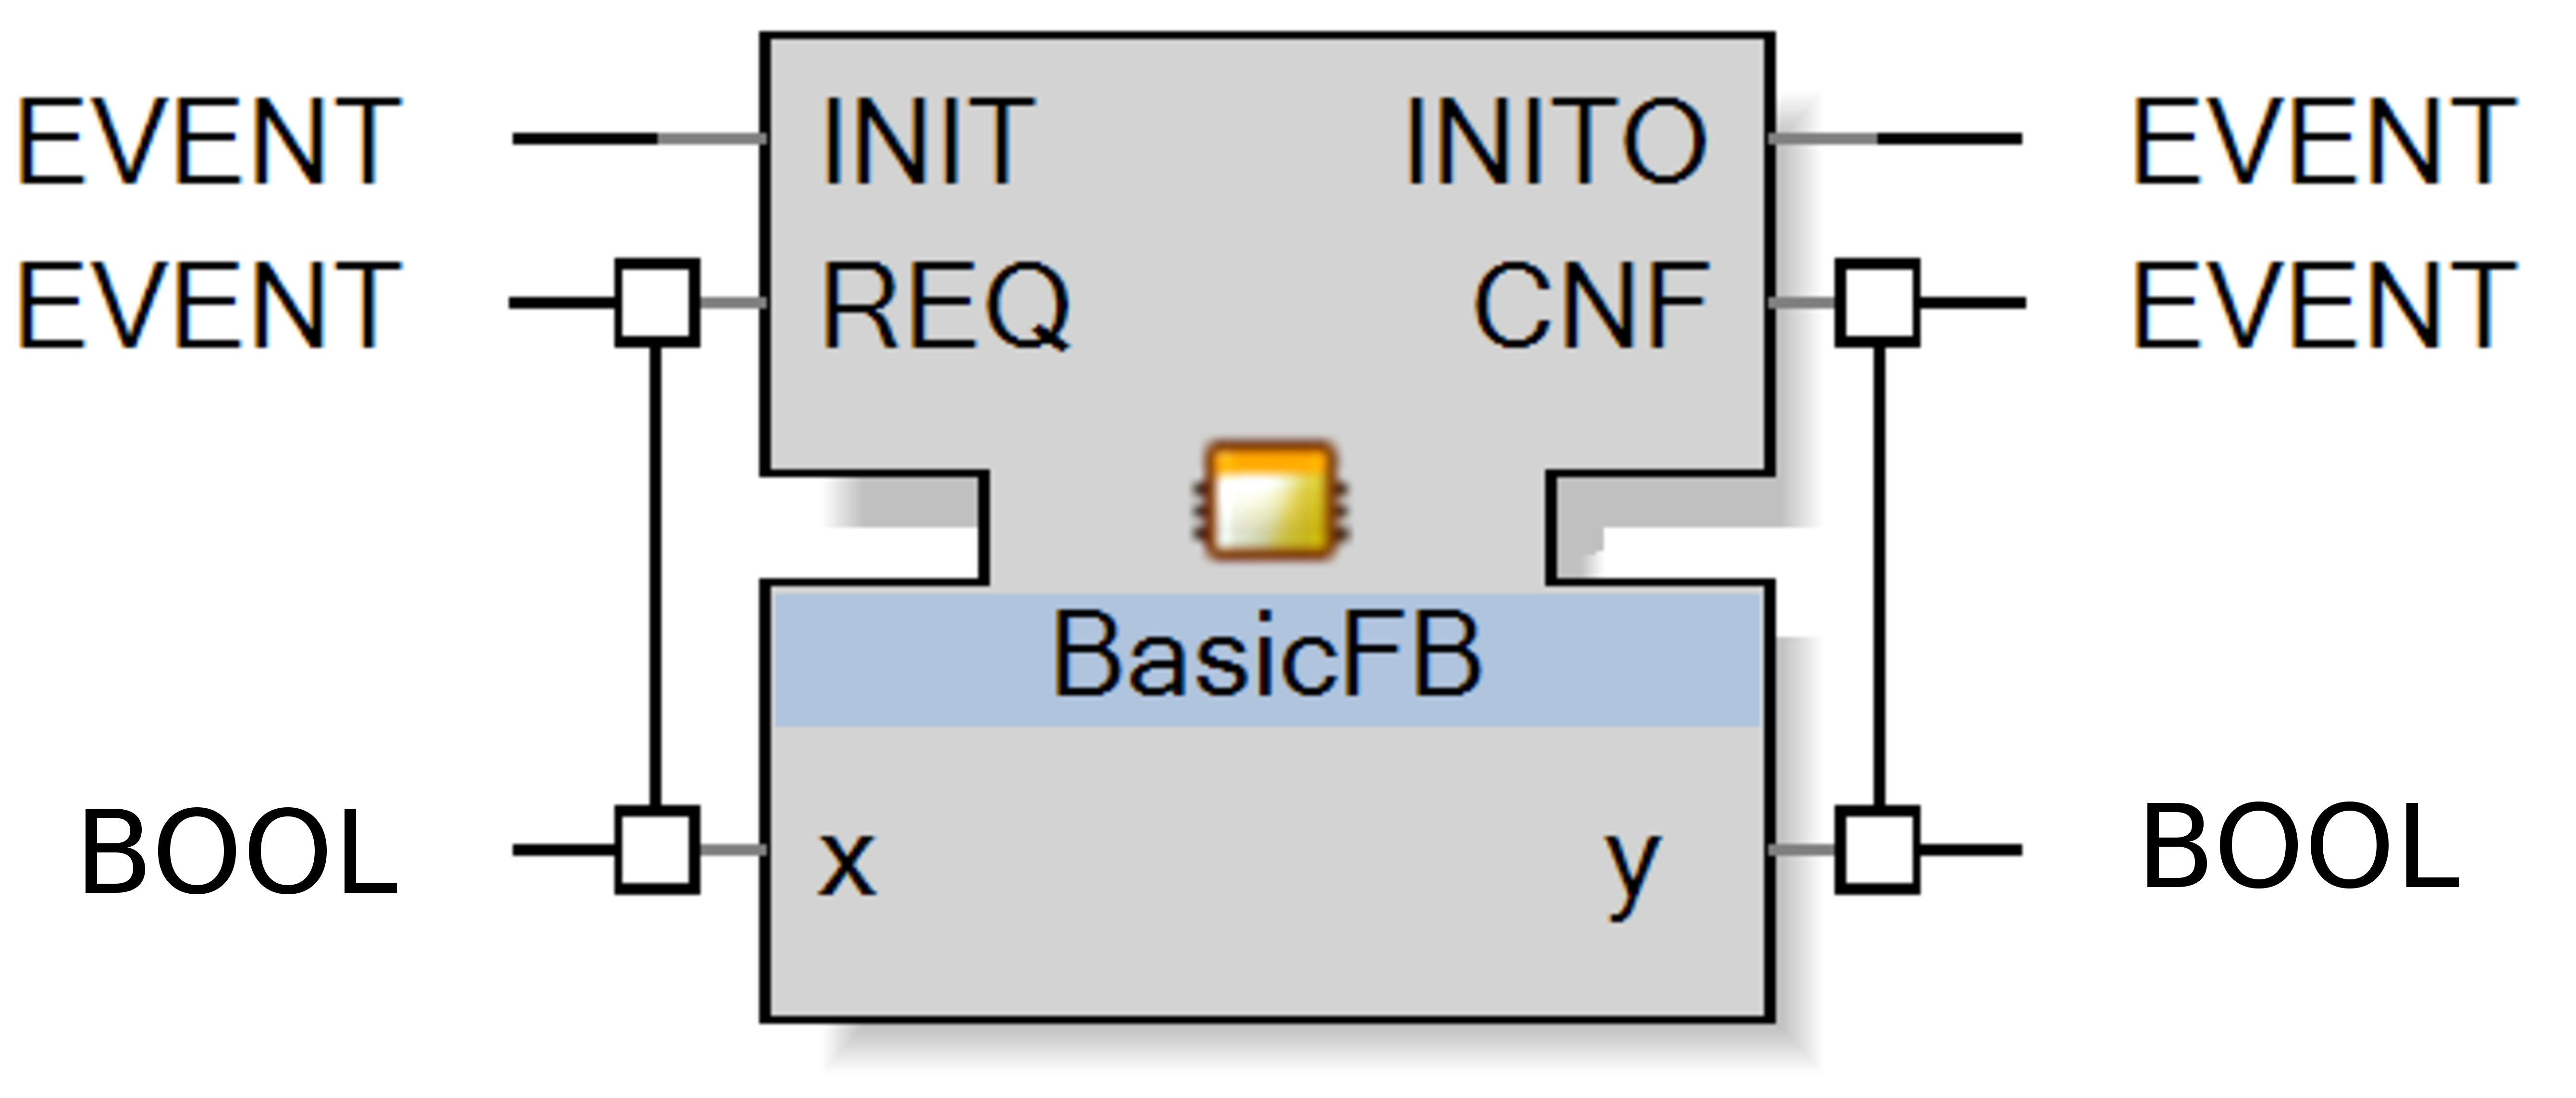
\includegraphics[width=2.5in]{pic/ecc-interface-bool.png}
    \caption{Пример интерфейса функционального блока}
    \label{fb-interface-example}
\end{figure*}

\begin{figure*}[t]
    \centering
    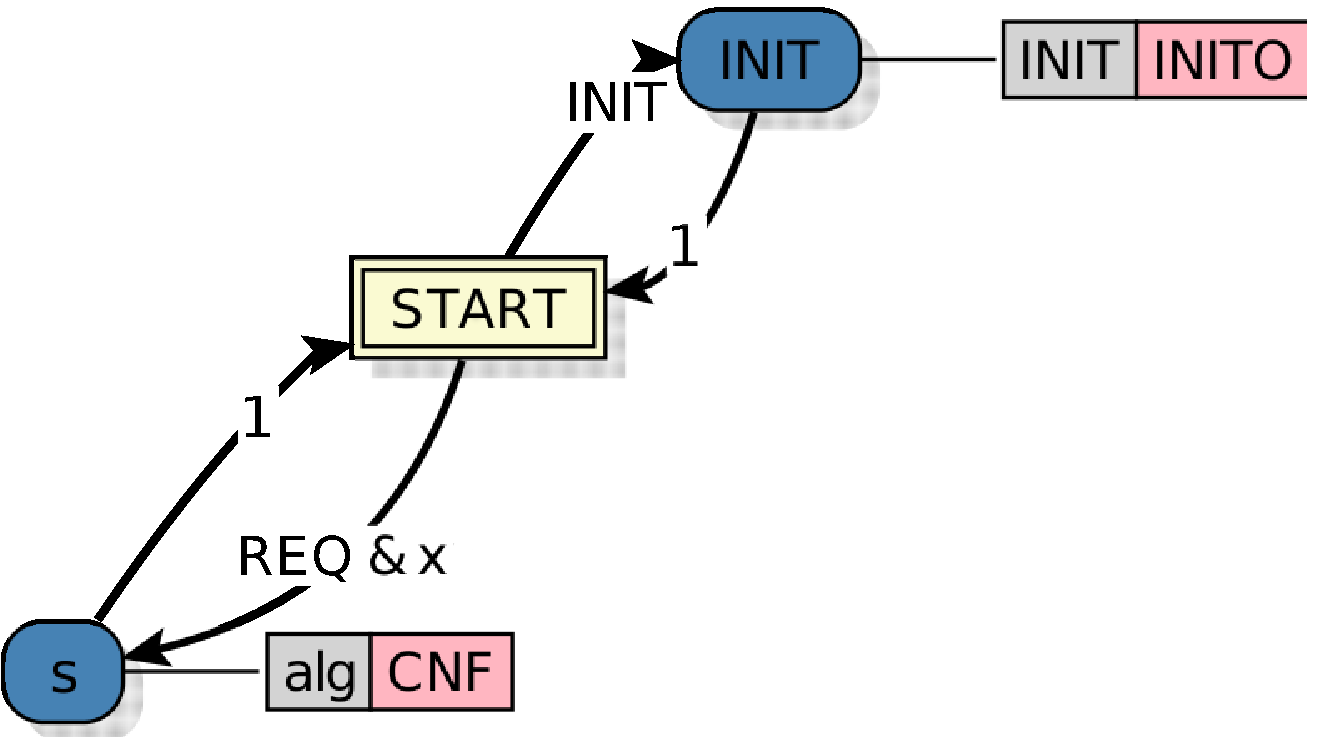
\includegraphics[width=2.5in]{pic/ecc-example-bool.png}
    \caption{Пример диаграммы управления выполнением функционального блока}
    \label{ecc-example}
\end{figure*}

\subsubsection{Темпоральные логики}

Темпоральная логика (\textit{temporal logic}) \cite{tl} --- это логика, учитывающая причинно-следственные связи в условиях времени.
Используется для описания последовательностей событий и их взаимосвязи по временной шкале.
Темпоральные логики часто применяются для выражения требований для формальной верификации.

Язык темпоральной логики состоит из зависящих от задачи
пропозициональных переменных, операторов булевой логики и набора темпоральных
операторов, таких как:

\begin{itemize}
    \item $G(f)$ означает, что формула $f$ должна выполняться во всех состояниях.
    \item $X(f)$ означает, что формула $f$ должна выполняться в следующем состоянии.
    \item $F(f)$ означает, что формула $f$ должна выполняться в каком-либо из будущих состояний.
\end{itemize}

Так как описываемая система может быть недетерминированой, то в каждом
состоянии могут существовать различные пути развития. В рамках логики
деревьев вычислений (\textit{computation tree logic, CTL}) допускается использование кванторов. Квантор $\forall$
требует, чтобы формула выполнялась на всех путях, исходящих из состояния, а
квантор $\exists$, чтобы существовал такой путь, на котором формула выполяется.
В рамках линейной темпоральной логики формула должна выполняться на всех путях.

Свойства систем можно разделить на два типа: функциональные свойства и свойства безопасности.
Функциональные свойства описывают корректное поведение системы, то есть то, что она должна делать,
а свойства безопасности -- некорректное, то есть, что она не должна делать. Если для примера рассмотреть работу лифта,
то свойство, утверждающее, что, будучи вызванным на некоторый этаж, лифт рано или поздно туда приедет, будет
функциональным свойством, а свойство запрещающее езду с открытыми дверями -- свойством безопасности.

\subsubsection{Сценарии работы}

Сценарий работы это последовательность четверок $\langle e, i, z, o
\rangle$, где $e : E$ -- входное событие, $i : \{0, 1\}^{|I|}$ -- вектор
значений входных переменных, $z : Z^*$ -- выходные события и $o :
\{0, 1\}^{|O|}$ -- вектор значений выходных переменных. Говорят, что диаграмма
управления выполнением в состоянии $S$ удовлетворяет элементу сценария, если, получив на вход
входное событие и значения входных переменных из элемента, она выдает выходные события и значения
выходных переменных из элемента. Говорят, что диаграмма управления выполнением удовлетворяет
сценарию если она удовлетворяет первому элементу сценария в своем начальном состоянии и для каждого
из последующих элементов сценария диаграмма управления выполнением удовлетворяет элементу в состоянии,
в которое она перешла после выполнения предыдущего элемента. 

\subsubsection{Методы генерации конечных автоматов без учета темпоральных формул}

Методы решения задачи генерации конечных автоматов, как точные так и эвристические, существуют уже достаточно давно.
Одной из первых работ принято считать статью, в которой было предложено моделировать эволюционные процессы для
создания предсказателей в форме конечных автоматов. Под конечным автоматом подразумевалась программа, в каждый момент времени
находящаяся в некотором состоянии. Прочитав входной символ, программа переходит в новое состояние и генерирует выходную строку.
Задачей автомата было предсказание символов строки, а функция приспособленности оценивала насколько хорошо автомат предсказывает данные.

Генетические алгоритмы применялись для решения задачи о флибах. Суть задачи состоит в построении автомата-преобразователя,
предсказывающего состояние некой среды, заданное битовой маской определенной длины. Генетические алгоритмы также применялись
для решения задачи об «Умном муравье». В \cite{ps, ask} генетические алгоритмы использовались для построения автопилота для
управления беспилотным летательным аппаратом.

Отметим, что когда число входных переменных автомата велико становится важным способ представления автоматов в виде особей
эволюционного алгоритма. Самым простам способом является метод полных таблиц переходов, в котором для каждой комбинации
значений входных переменных хранится переход. Подобный спопоб, однако, чрезмерно затратен и приводит к снижению производительности
в случае большого числа входных переменных. Поэтому в был разработан метод сокращенных таблиц переходов, в котором хранятся
переходы только для выбранного множества значимых входных переменных.

В \cite{sat} предложено сведение задачи генерации детерминированных конечных автоматов
к задаче выполнимости булевых формул (SAT). Позже, в работе \cite{csp} был предложен алгоритм, основанный на сведении к задаче
удовлетворения ограничениям (CSP).

\subsubsection{Методы генерации конечных автоматов с учетом темпоральных формул}

\subsubsection{Постановка задачи}

Будем называть исходным некоторый функциональный блок $M$, восстановление логики которого нас интересует.
Пусть $F$ -- набор формул линейной темпоральной логики, которым удовлетворяет исходный блок,
а $S$ -- набор сценариев, полученных при тестировании исходного блока.
Отметим, что алгоритм предложенный в данной работе не зависит от способа получения сценариев.
Метод тестирования функциональных блоков выходит за рамки данной работы.
Нашей целью является нахождение такого автомата $M_1$, что выполяются следующие условия.

1) $M_1$ удовлетворяет всем формулам из $F$.

2) $M_1$ удовлетворяет всем сценариям из $S$.

\subsection{Обзор используемых подходов}
\subsubsection{Верификация символьных моделей}

Верификация используется для проверки систем с
конечным числом состояний на то, удовлетворяют ли они заданным темпоральным
свойствам. Метод символьной верификации используется для борьбы с чрезмерным числом состояний модели. В рамках данного метода вместо построения графа
состояний используются булевы формулы, представляющие множества и отношения, а свойства проверяются непосредственно
через манипуляции с этими формулами. В языке SMV (symbolic model verification) переменные принадлежат конечным скалярным типам, а
программы состоят из параллельных операторов присвоения. Таким образом
программа может рассматриваться как система уравнений, а ее решением будет
следующее состояние модели. При этом запрещены множественное присвоение одной
переменной и циклические зависимости, что позволяет гарантировать, что решение
существует. Заметим так же, что решений может быть несколько, в этом случае имеет
место недетерменированное поведение.

\subsubsection{Восстановление логики функциональных блоков с использованием
метаэвристического алгоритма}

Так как предлагаемый подход основан на \cite{rec}, мы приведем краткий обзор метода синтеза
блоков из указанной работы. Этот метод основан на метаэвристической
оптимизации. Метаэвристические алгоритмы используются для нахождения хороших
решений сложных задач (например тех, для которых нахождение точного решения
вычислительно сложно) за разумное время.

Процесс поиска в \cite{rec} начинается с генерации случайных начальных решений-кандидатов
(случайных диаграмм управления выполнением). Затем пространство поиска,
которое является множеством всех возможных диаграмм с фиксированным интерфейсом и числом состояний,
исследуется с помощью так называемых операторов мутации: процедур, которые
вносят некоторые изменения в структуру диаграмм. Например в \cite{rec} используются
следующие операторы:

1) Выбрать случайный переход и изменить состояние, в которое он ведет.

2) Выбрать случайный переход и удалить его.

3) Выбрать случайное состояние и добавить переход в другое случайное состояние.

Каждое новое решение-кандидат затем оценивается при помощи функции приспособленности:
она измеряет насколько хорошо решение удовлетворяет сценариям. Это происходит
следующим образом. Каждый сценарий обрабатывается отдельно. На вход
диаграмме управления выполнением подаются входные значения из элементов
сценария, а выходные значения записываются. Затем значения, сгенерированные
диаграммой, сравниваются с соответствующими значениями сценария, с помощью
расстояния Левенштейна. Результаты нормализуются по отношению к длине сценария
и усредняются по всем сценариям. Функция приспособленности также измеряет
некоторые другие параметры: позицию первой ошибки (чем больше -- тем лучше) и
число переходов из одного состояния в другое в процессе исполнения (чем меньше
-- тем лучше).

Функция приспособленности выглядит следующим образом:
$$
F = c_1 F_{ed} + c_2 F_{fe} + c_3 F_{sc},
$$
где $F_{ed}$ основано на расстоянии Левенштейна, $F_{fe}$ на позиции первой
ошибки и $F_{sc}$ на числе смен состояний, а $c_1, c_2, c_3$ -- константы.
Алгоритм оптимизации пытается максимизировать данную функцию.

\subsubsection{Верификация в открытом и замкнутом цикле}

Промышленные приложения обычно состоят из объекта управления и системы управления.
Существует два основных подхода к верификации систем управления --
верификация открытого цикла и верификация замкнутого цикла \cite{cl}. В верификации
открытого цикла система управления верифицируется изолированно. Наоборот, в
верификации замкнутого цикла производится одновременная верификация системы управления
и модели объекта управления. Второй подход более логичен чем первый, поскольку
интерес представляет поведение системы управления при работе с объектом управления. Более того, в
верификации открытого цикла мы можем не иметь возможности верифицировать
некоторые верные утверждения так как ничто не ограничивает поведение объекта управления.
Также заметим, что некоторые свойства принципиально не могут быть проверены при
верификации с открытым циклом.

Однако, у верификации замкнутого цикла есть серьезная проблема -- нам нужна не
только формальная модель системы управления, но еще и формальная модель объекта управления.
В некоторых случаях модель объекта управления также может быть сгенерирована
автоматически \cite{dd}, но это может привести к очень большим моделям, которые будет
сложно верифицировать. Например даже при использовании абстракции объекта управления \cite{dd},
верификация замкнутого цикла для механического манипулятора заняла
294 секунды. Учитывая то, что в нашей работе нам придется верифицировать
большое число решений-кандидатов, такие временный затраты на верификацию неприемлимы.

\subsection{Предлагаемый подход}

Для решения поставленной задачи предлагается следующий подход.  В его основе лежит параллельный
метод оптимизации, предложенный в \cite{rec}. Алгоритм дополняется с помощью новых
составляющих функции приспособленности и оператора мутации. Верификация
решений-кандидатов основана на использовании суррогатной модели объета управления, что сильно уменьшает время,
необходимое на верификацию. Мы используем программное средство NuSMV \cite{nusmv} для верификации SMV-моделей
функциональных блоков.

\subsubsection{Верификация в замкнутом цикле с использованием суррогатной модели
объекта управления}

Подход, представленный в данной работе, лежит между верификацией открытого и
замкнутого цикла. Опишем процессы создания моделей.

1) Модель системы управления. Создадим переменную $eccState : Y$ чтобы хранить
состояние системы. Для каждого входного и выходного события создадим
булеву переменную, указывающую -- произошло событие или нет. Для каждой из
входных и выходных переменных создадим соответствующую ей переменную.

Изначально в $eccState$ записано начальное состояние диаграммы. Затем, на
каждом шаге будем обновлять ее состояние исходя из ее текущего состояния,
входных событий и значений входных переменных. Выходные события и значения
выходных переменных вычисляются исходя из нового значения $eccState$. Выходные
действия могут заключаться в генерации выходного события, установки значения
выходной переменной в $true$, установки значения выходной переменной в $false$
или сохранении текущего значения переменной.

2) Суррогатная модель объекта управления. Затем вручную создается суррогатная модель
объекта управления и окружения и соединяется с моделью системы управления. Все, что
требуется от заменителя, это то, он будет взаимодействовать с системой управления так,
как это делают реальные объект управления и окружение. Все другие детали избыточны. Это
значит, что заменитель модели может быть гораздо проще чем реальная модель
установки и окружения, что сильно ускоряет верификацию. Недостатком данного
подхода является то, что необходимо построить этот заменитель, что может быть
нетривиальной задачей.

\subsubsection{Функция приспособленности}

Получив спецификацию, состоящую из формул темпоральной логики, NuSMV проверяет
удовлетворяет ли данная SMV-модель спецификации. Для каждой формулы он сообщает
либо то, что она удовлетворена, либо контрпример как доказательство того, что
она не удовлетворена.

Первая компонента функции приспособленности $F^{sat}_{smv}$ измеряет
отношение числа удовлетворенных формул к общему их числу. Этого, однако, недостаточно
так как получить решение, удовлетворяющее большему числу формул, чем имеющиеся на данный
момент решения, мы можем лишь благодаря случайности, что может занять очень большое количество времени.
Поэтому будем использовать в нашем алгоритме контрпримеры. Использование контрпримеров
вынуждает нас ограничиться линейной темпоральной логикой, исключив логику
деревьев вычислений. Это связано с тем, что для тех формул логики деревьев
вычислений, которые используют экзистенциальную квантификацию и не выполняются,
мы не можем привести контрпример так как нет такого примера, который бы
доказывал, что некоторого пути не существует.

Будем использовать дополнительную компоненту $F^{ce}_{smv}$, которая
основана на длине наиболее длинного контрпримера $l_{max}$ для
неудовлетворенной формулы. Идея, которая стоит за этим, заключается в том, что
решения с более длинными контрпримерами скорее всего лучше, чем решения с
короткими. Так как максимальной длины контрпримера не существует, мы
воспользуемся слудующей формулой.
$$
F^{ce}_{smv} = \begin{cases} 1, & \mbox{если}\ l_{max} = 0 \\
1 - \frac{1}{(1 + \frac{1}{10}l_{max})^{\frac{1}{10}}}, & \mbox{иначе}
\end{cases}
$$
Значение $F^{ce}_{smv}$ равно единице, когда $l_{max} = 0$ и стремится к
единице, когда $l_{max} \rightarrow 1$, что и требуется. Подводя итог,
новая функция приспособленности имеет вид:
$$
F = c_1 F_{ed} + c_2 F_{fr} + c_3 F_{sc} + c_4 F{sat}_{smv} + c_5 F^{ce}_{smv}.
$$

Проблема с использованием верификации в функции приспособленности заключается
в том, что даже несмотря на то, что мы не используем полную модель объекта управления,
время, необходимое на верификацию, значительно больше, чем время, необходимое
для вычисления других компонент функции приспособленности. Для решения данной проблемы
предлагается следующий подход.

Вместо того чтобы вычислять компоненты, основанные на верификации, для каждого
решения, мы будем вычислять их с некоторой вероятностью $p$, а с вероятностью
$1 - p$ использовать значения, вычисленные для предка решения. Конечно, это
может привести к потере некоторых хороших решений, однако такова цена.

Так же, если сумма остальных компонент выше некоторого порогового значения, то всегда
будем производить верификацию. Это позволяет нам избежать потери близких к оптимальному
решений и гарантирует, что финальное решение действительно удовлетворяет
поставленной задаче.

\subsubsection{Оператор мутации, использующий контрпримеры}

Как уже было отмечено ранее, в случае, если решение не удовлетворяет LTL-формуле,
NuSMV предоставляет контрпример. Контрпример можно рассматривать как сценарий
работы. В добавление к тому, что мы используем контрпримеры в функции
приспособленности, так же будем использовать их в специальном операторе
мутации, похожем на предложенный в \cite{et} для управления конечным автоматом. Особенность данного оператора является повышение вероятности
удаления или изменения переходов, входящих в контрпример.

Каждому переходу присваивается вес. Изначально вес каждого перехода равен
единице. Затем просмотрим все контрпримеры и, каждый раз используя некоторый переход,
будем увеличивать его вес на величину $\lambda$. Затем воспользуемся методом
рулетки с вероятностями, пропорциональными весам, для того чтобы выбрать
переход и изменить его конечное состояние на случайное.

\subsection{Вычислительные эксперименты}

\begin{figure}[t]
    \centering
    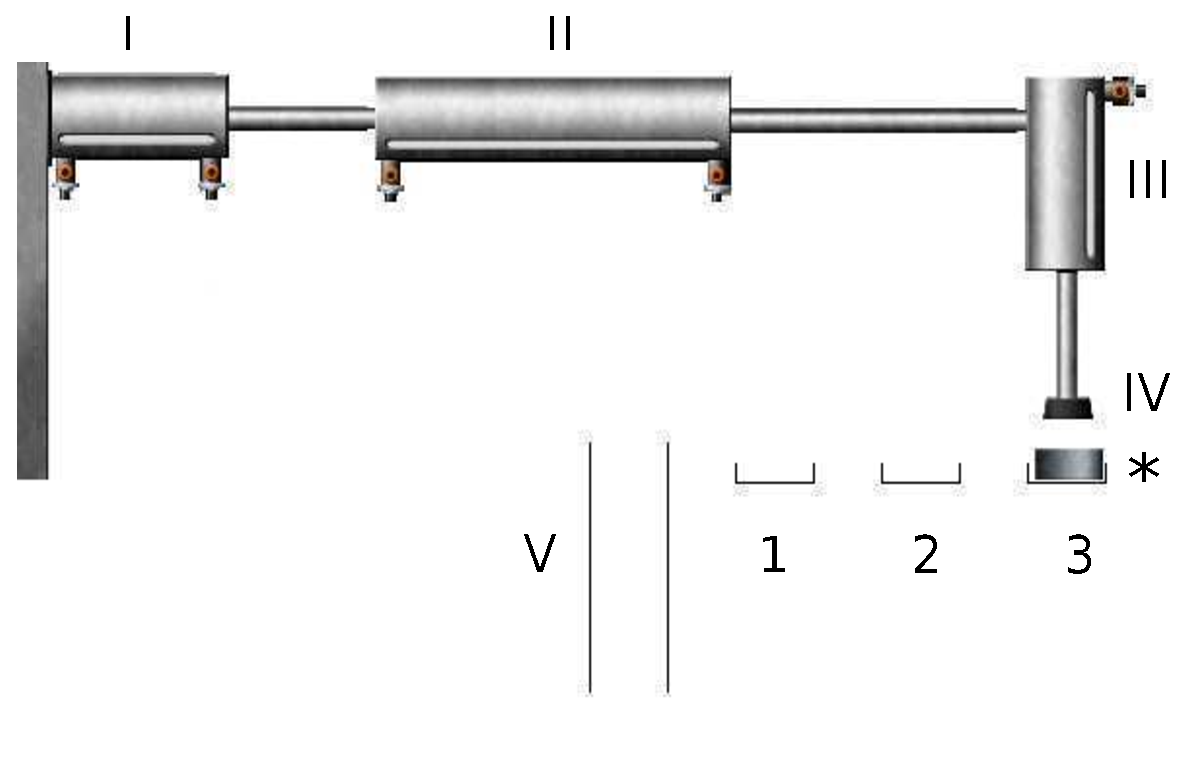
\includegraphics[width=3in]{pic/pnp.eps}
    \caption{PnP-манипулятор с тремя цилиндрами}
    \label{pnp-system}
\end{figure}

Для тестирования предлагаемого подхода был использован PnP-манипулятор \cite{pnp},
показанный на рисунке \ref{pnp-system}.
Он представляет собой механическую руку, три входных и одну выходную дорожку.
Рука состоит из двух горизонтальных цилиндров, которые могут выдвигаться и
вдвигаться. Один из горизонтальныз цилиндров больше по размеру и может выдвигаться
на большую длину, таким образом, четыре возможных комбинации позволяют позиционироваться над
каждой из четырех дорожек.

В состав руки так же входит вертикальный цилиндр, который позволяет
перемещать всасывающее устройство вверх и вниз. Оно используется чтобы
поднимать детали с дорожек и удерживать их. У манипулятора есть сенсоры, которые определяют
положения цилиндров, находится ли что-то на входных дорожках, а так же
захвачено ли что-нибудь рукой. Задача манипулятора перемещать детали с входных
дорожек на выходную.

На рисунке \ref{pnp-system} горизонтальные цилиндры отмечены как I и II,
вертикальный цилиндр -- III, всасывающее устройство -- IV, выходная дорожка -- V.
Три входных дорожки помечены цифрами 1, 2, 3.

\subsubsection{Модель объекта управления и среды}

Для каждой входной дорожки создадим две булевы переменных $p_i$ и $pp_i$.
Значения $p_i$ не ограничиваются, таким образом они моделируют
недетерменированное появление деталей, а значения $pp_i$ определяются
следующим образом. Если в данный момент рука поднимает деталь с $i$-ой
дорожки, то $pp_i := false$, если $pp_i = true$, то ее значение сохраняется,
иначе $pp_i := p_i$. Таким образом мы моделируем поведение, когда деталь
может появиться на дорожке в произвольный момент времени, но появившись
остается там до тех пор, пока не будет захвачена рукой.

Всасывающее устройство моделируется единственной переменной $v$, указывающей
включено устройство или выключено. Если система управления подает команду включить
или выключить устройство, мы изменяем переменную соответствующим образом,
иначе оставляем ее нетронутой.

Так как цилиндры двигаются не мгновенно, для каждого из них создадим переменную
$cs_i : \{cst_j | j = 0 .. 3 \}$, хранящую состояние цилиндра. Будем изменять
эти переменные в соответствии с командами системы управления. В свою очередь сенсоры
будут использовать эти переменные для определения положения цилиндра.

Последнее, что остается сделать -- это задать работу индикатора того, держит
ли рука что-нибудь или нет. Для этого создадим переменную $vac$. Алгоритм
ее вычисления прост. Если всасывающее устройство выключено, то
$vac := false$, если всасывющее устройство расположено над дорожкой с деталью,
вертикальный цилиндр выдвинут и устройство включено, то $vac := true$, иначе
ее значение сохраняется.

Общая схема работы модели такова. На каждом шаге генерируется входное событие
и подаем запрос на пересчет своего состояния. Это происходит в соответствии с диаграмой
управления выполнением, текущим состоянием модели и значениями входных
переменных. Затем мы пересчитываем состояние окружения исходя из его текущего
состояния, значений выходных переменных контроллера и вышеуказанных правил.

\subsubsection{Эксперименты}

Наши эксперименты преследовали несколько целей. Во-первых, проверить и
продемонстрировать практическую применимость предлагаемого подхода, а, во-вторых,
проверить, что использование длины контрпримеров в функции приспособленности
приводит к улучшению работы алгоритма.

Использовался один сценарий работы, соответствующий обработке одной детали на
первой дорожке. Длина этого сценария 2339. Так же были использованы
следующие три темпоральных свойства:
\begin{enumerate}
    \item $G(\lnot (c1Extend \wedge c1Retract))$~-- свойство безопасности, гласящее, что
первый цилиндр не должен получать команд на выдвижение и вдвижение одновременно;
    \item $G(\lnot (c2Extend \wedge c2Retract))$~-- аналогичное свойство для второго цилиндра;
    \item $G(pp1 \rightarrow F(vp1))$~-- функциональное свойство, гласящее, что, если деталь
появилась на первой дорожке, то когда-нибудь она будет обработана.
\end{enumerate}

Алгоритм был реализован\footnote{\url{https://github.com/V1489Cygni/spec2fb}} на языке Java.
Использовалось программное средство NuSMV 2.5.4 для верификации
темпоральных свойств, NuSMV запускалось с параметрами по умолчанию. Все эксперименты
проводились на машине с 64-ядерным процессором AMD Opteron\texttrademark 6378 @ 2.4 ГГц.
Использовались 16 ядер и 32 гигабайта оперативной памяти.

Сперва в качестве входных данных использовался только сценарий. Было проведено 50 запусков.
Затем были проведены запуски, с использованием темпоральных свойств, но не без использования длины
контрпримеров в функции приспособленности. Наконец были проведены запуски с верификацией и использованием контрпримеров.
Результаты запусков приведены в таблице \ref{results-table}.

\begin{table*}[t]
\centering
\caption{Экспериментальные результаты}
\label{results-table}
\begin{tabular}{c|c|c|c|c|c|c}
\hline
\# & Конфигурация & \multicolumn{4}{c|}{Время, с} & Доля удовлетворенных формул\\
\hline
 &              & мин & средн & мед & макс & \\
\hline
1 & Сценарии                            & 32       & 85        & 81          & 280  & 0\%\\
2 & Сценарии + LTL (без $F_{smv}^{ce}$) & 222      & 752       & 656         & 1689 & 100\%\\   
3 & Сценарии + LTL                      & 164      & 563       & 561         & 1575 & 100\%\\
\hline
\end{tabular}
\end{table*}

Во-первых, отметим, что все сгенерированные решения удовлетворяли первым двум
темпоральным свойствам. Это было ожидаемо так как это свойства безопасности ---
они описывают что система делать не должна. Они могут быть удовлетворены даже
если система ничего не делает.

Во-вторых, ни одно из сгенерированных без темпоральных формул решений не удовлетворило
третьей формуле. Это подтверждает, что весьма маловероятно, что можно случайно
сгенерировать решение, удовлетворяющее функциональным темпоральным свойствам.

В-третьих, использование верификации в функции приспособленности привело
к генерации решений, которые удовлетворяли всем формулам. Так же очевидно, что использование
верификации привело к значительному увеличению времени работы алгоритма. В свою очередь,
использование длины контрпримеров в функции приспособленности привело к ускорению на 30\%.

После генерации все решения было проверены в системе моделирования FBDK\footnote{\url{http://www.holobloc.com/doc/fbdk}}.
Все решения, сгенерированные с учетом темпоральных свойств успешно обрабатывали дорожку несколько раз,
в то время как решения, сгенерированные только по сценарию, не обрабатывали ее более одного раза.

\subsection{Заключение}

В данной работе был предложен подход для генерации простых функциональных блоков по
сценариям работы и темпоральным свойствам. Верификация была встроена в функцию приспособленности и
оператор мутации. Верификация проводится по способу замкнутого цикла с использованием
созданной вручную модели среды и объекта упраления. Эта модель отображает внешнее поведение
объекта управления и гораздо проще чем полная модель.

Вычислительные эксперименты подтвердили применимость предлагаемого подхода, сгенерировав диаграммы управления состоянием для
описанного PnP-манипулятора, которые выполняли поставленную задачу --- перемещать детали
с входной дорожки на выходную. При помощи добавления верификации мы смогли гарантировать,
что такое поведение будет наблюдаться необходимое число раз, что не наблюдается в
результатах полученным лишь по сценариям.

По резуль татам данной работы была написана и принята на конференцию статья \cite{this}.

\pagebreak

\begin{thebibliography}{99}
\addcontentsline{toc}{subsection}{Литература}

\bibitem{iec}
V. Vyatkin, “IEC 61499 as Enabler of Distributed and Intelligent
Automation: State-of-the-Art Review,” IEEE Transactions on Industrial
Informatics, vol. 7, no. 4, pp. 768–781, Nov 2011.

\bibitem{rec}
D. Chivilkhin, A. Shalyto, S. Patil, and V. Vyatkin, “Reconstruction of
function block logic using metaheuristic algorithm: Initial explorations,”
in Proceedings of IEEE International Conference on Industrial Informat-
ics, 2015, pp. 1239–1242.

\bibitem{ea}
T. Back, D. B. Fogel, and Z. Michalewicz, Eds., Handbook of Evolu-
tionary Computation. Bristol, UK: IOP Publishing Ltd., 1997.

\bibitem{cl}
V. Vyatkin, H.-M. Hanisch, C. Pang, and C.-H. Yang, “Closed-loop
modeling in future automation system engineering and validation,”
Systems, Man, and Cybernetics, Part C: Applications and Reviews, IEEE
Transactions on, vol. 39, no. 1, pp. 17–28, Jan 2009.

\bibitem{dd}
S. Patil, D. Drozdov, V. Dubinin, and V. Vyatkin, Technological
Innovation for Cloud-Based Engineering Systems: 6th IFIP WG
5.5/SOCOLNET Doctoral Conference on Computing, Electrical and
Industrial Systems, DoCEIS 2015, Costa de Caparica, Portugal, April
13-15, 2015, Proceedings. Cham: Springer International Publishing,
2015, ch. Cloud-Based Framework for Practical Model-Checking of
Industrial Automation Applications, pp. 73–81. [Online]. Available:
http://dx.doi.org/10.1007/978-3-319-16766-4 8

\bibitem{nusmv}
A. Cimatti, E. Clarke, E. Giunchiglia, F. Giunchiglia, M. Pistore,
M. Roveri, R. Sebastiani, and A. Tacchella, “NuSMV Version 2: An
OpenSource Tool for Symbolic Model Checking,” in Proc. International
Conference on Computer-Aided Verification (CAV 2002), ser. LNCS, vol.
2404. Copenhagen, Denmark: Springer, 2002.

\bibitem{pnp}
S. Patil, V. Vyatkin, and M. Sorouri, “Formal verification of Intelligent
Mechatronic Systems with decentralized control logic,” in Proceedings
of the 17th IEEE Conference on Emerging Technologies Factory Au-
tomation, 2012, pp. 1–7.

\bibitem{et}
F. Tsarev and K. Egorov, “Finite state machine induction using genetic
algorithm based on testing and model checking,” in Proceedings of
the 13th Annual Conference Companion on Genetic and Evolutionary
Computation, ser. GECCO ’11. New York, NY, USA: ACM, 2011, pp.
759–762.

\bibitem{tl}
A. Pnueli. The temporal logic of programs.
In Foundations of Computer Science, 1977., 18th Annual Symposium on, pages 46–57, Oct 1977.

\bibitem{this}
Chivilikhin D., Ivanov I., Shalyto A., Vyatkin V. Reconstruction of Function Block
Controllers Based on Test Scenarios and Verification / To appear in Proceedings of
the 14th IEEE International Conference on Industrial Informatics, 2016.

\bibitem{ps}
Поликарпова Н. И., Точилин В. Н., Шалыто А. А.
Метод сокращенных таблиц для генерации автоматов с большим числом входных
переменных на основе генетического программирования // Известия РАН.
Теория и системы управления. — 2010. — № 2. — С. 100—117.

\bibitem{ask}
Genetic algorithm for induction of finite automata with continuous and
discrete output actions / A. Alexandrov, A. Sergushichev, S. Kazakov,
F. Tsarev // Proceedings of the 13th annual conference companion on
Genetic and evolutionary computation. — New York, NY, USA : ACM,
2011. — P. 775–778.

\bibitem{sat}
Heule M., Verwer S. Exact DFA Identification Using SAT Solvers // Proceedings
of the 10th International Colloquium Conference on Grammatical
Inference: Theoretical Results and Applications. — Berlin, Heidelberg
: Springer-Verlag, 2010. — P. 66–79.

\bibitem{csp}
Chivilikhin D., Ulyantsev V., Shalyto A. Combining Exact and Metaheuristic
Techniques for Learning Extended Finite-State Machines from
Test Scenarios and Temporal Properties // Proceedings of the 13th International
Conference on Machine Learning and Applications. — IEEE
Computer Society, 2014. — P. 350–355.

\bibitem{meh}
Blum C., Roli A. Metaheuristics in Combinatorial Optimization: Overview and
Conceptual Comparison // ACM Comput. Surv. -- New York, NY, USA, 2003. --
Vol. 35, no. 3. -- P. 268-308.

\end{thebibliography}

\end{document}
